%%%%%%%%%%%%%%%%%%%%%%%%%%%%%%%%%%%%%%%%%%%%%%%%%%%%%%%%%%%%%%%%%%%%%%%%
\chapter{Motivation}
%%%%%%%%%%%%%%%%%%%%%%%%%%%%%%%%%%%%%%%%%%%%%%%%%%%%%%%%%%%%%%%%%%%%%%%%

%%%%%%%%%%%%%%%%%%%%%%%%%%%%%%%%%%%%%%%%%%%%%%%%%%%%%%%%%%%%%%%%%%%%%%%%
\section{GNN Inference Challenges and Opportunities}
%%%%%%%%%%%%%%%%%%%%%%%%%%%%%%%%%%%%%%%%%%%%%%%%%%%%%%%%%%%%%%%%%%%%%%%%
Although GNN inference has similarity to training, inference has unique challenges and opportunities not present in the training setting. 
In this section we examine these differences in detail, discuss inference bottlenecks based on concrete experiments, and motivate our approach based on an analysis of naive solutions.

\subsection{Inference-specific Challenges}
Leveraging approaches from existing training systems present several key challenges, namely:

\begin{enumerate}
    \item \textbf{Latency is a key metric at inference time}. This is not the case during training. During training, throughput is a far more important metric than latency. For example, many training systems avoid data loading bottlenecks using pipelining. However, pipelining cannot hide latency.
    \item \textbf{Node ordering cannot be controlled}. While training systems can use 
    \item \textbf{No backpropagation leads to sampling and data loading dominating inference latency}. 
\end{enumerate}

\begin{figure}[h!]
    \centering
    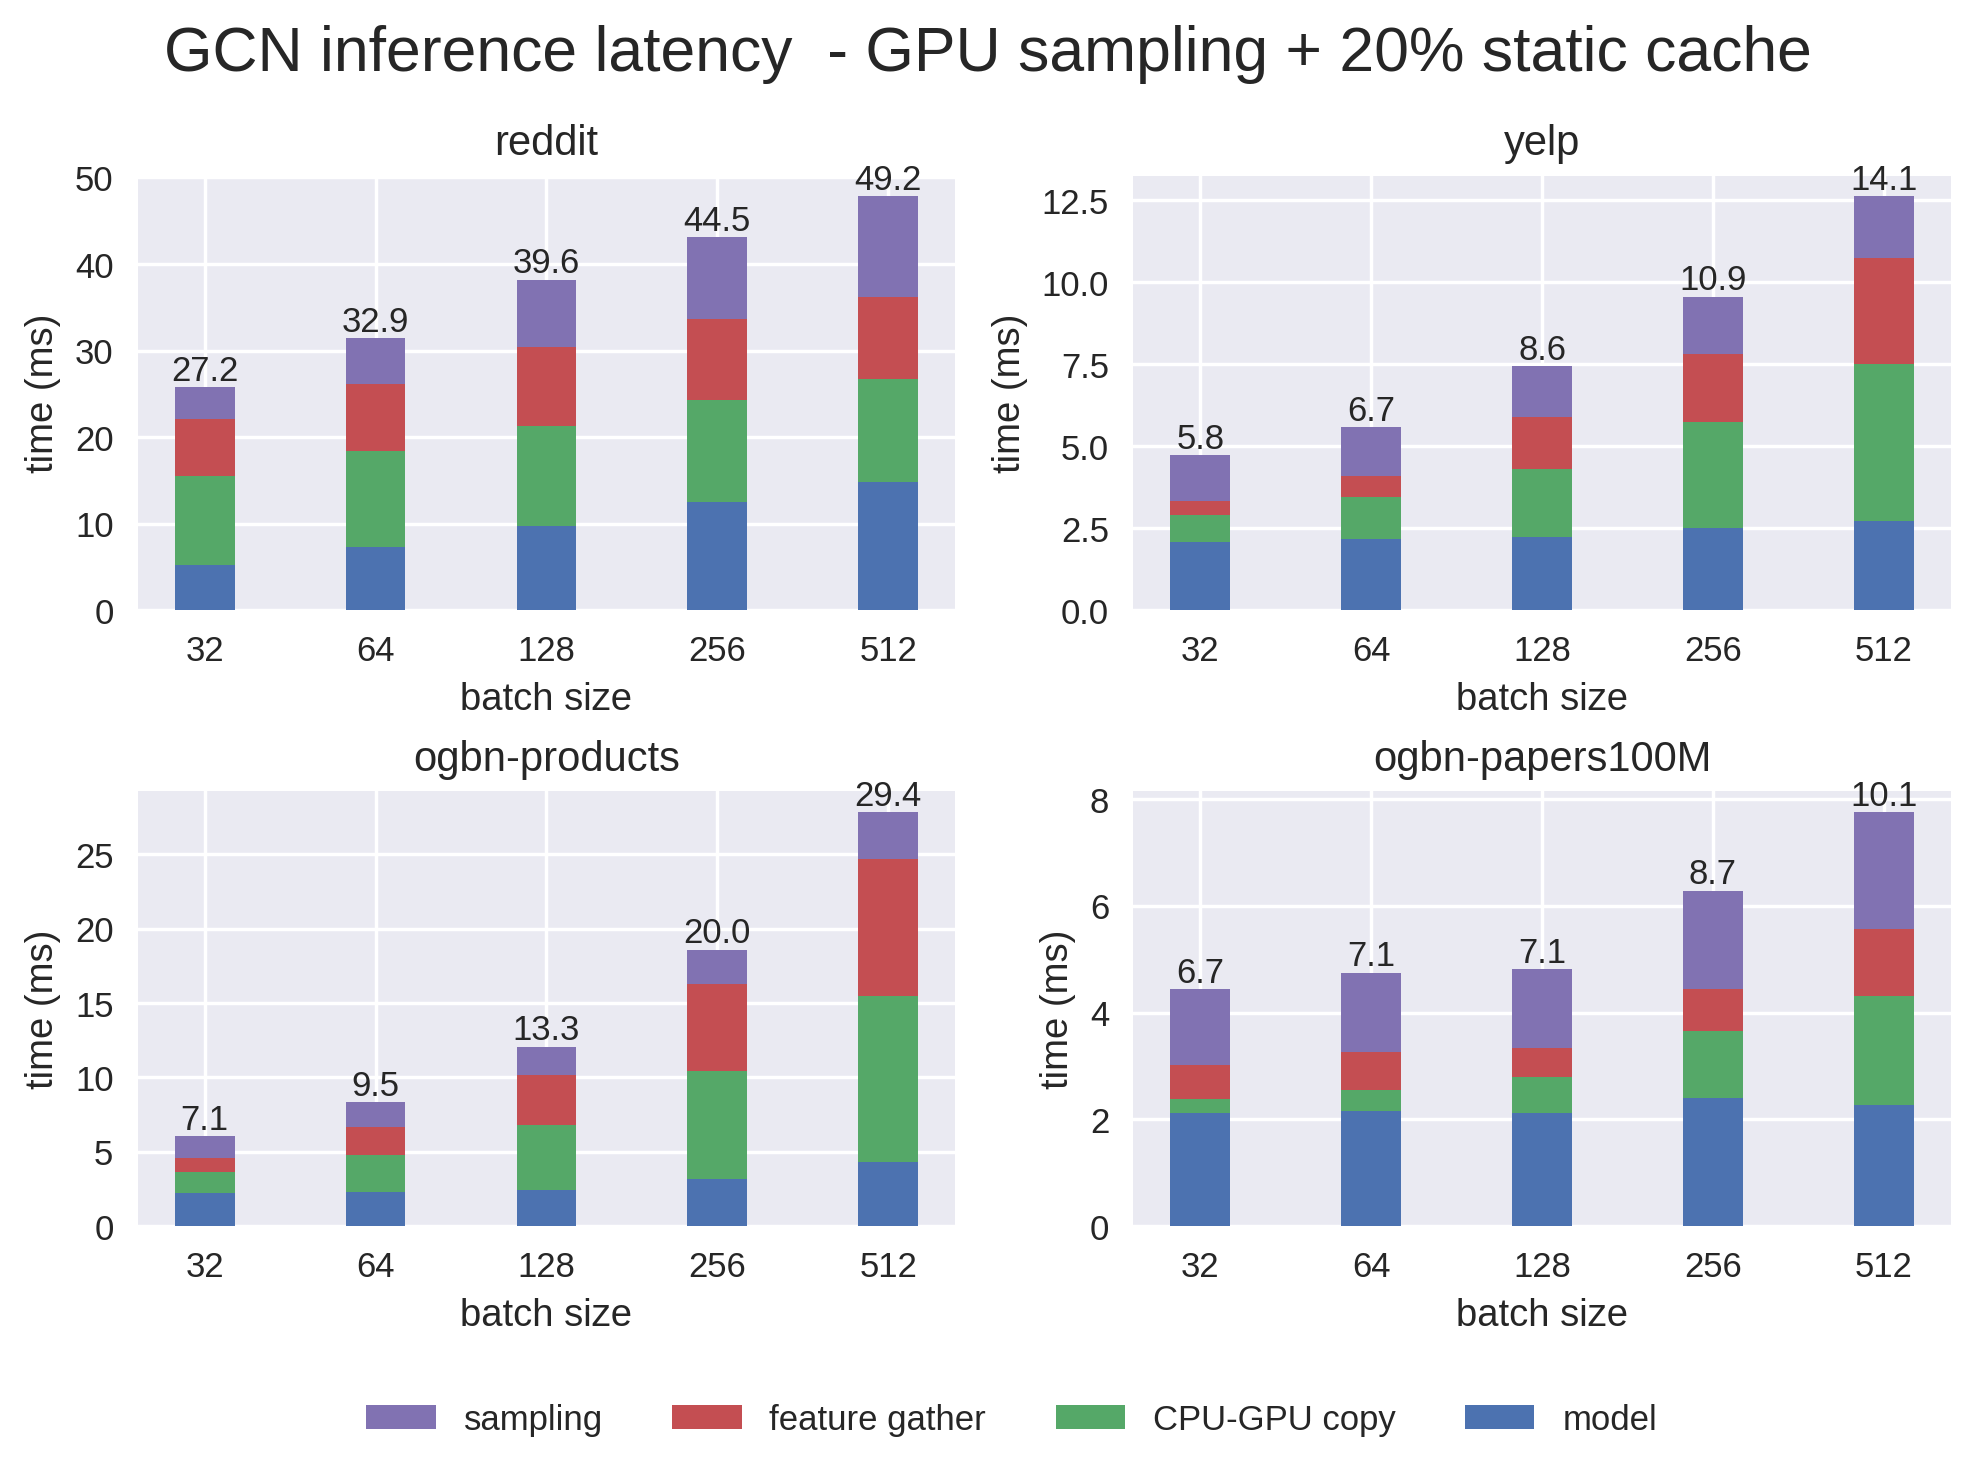
\includegraphics[width=\textwidth]{figures/GCN_latency_breakdown_gpu_sampled_with_cache.png}
    
    \caption{Inference latencies for different graph datasets and request batch sizes (number of target nodes in request). Requests are served by a system using GPU sampling and a static cache large enough to hold 20\% of the graph's node features.}
    \label{GPU Sampling Latency Breakdown}
\end{figure}    

\begin{enumerate}
    \item Inference latency is important, here is example
    \item Existing solutions don't work for inference \& 
         Data loading is the bottleneck after using GPU sampling
    \item Subgraph locality opportunity means we can exploit dynamic cache
    \item Challenging because need to meet latency and throughput SLAs
    \item Go into our solution
\end{enumerate}

% %%%%%%%%%%%%%%%%%%%%%%%%%%%%%%%%%%%%%%%%%%%%%%%%%%%%%%%%%%%%%%%%%%%%%%%%
% \section{Towards Dynamic Caching}
% %%%%%%%%%%%%%%%%%%%%%%%%%%%%%%%%%%%%%%%%%%%%%%%%%%%%%%%%%%%%%%%%%%%%%%%%


\subsection{Subgraph Locality of Inference Requests}
% Discuss when and why inference requests may have locality
Our key observation is that inference requests can 

\subsection{Naive Approaches to Dynamic Caching}
% Explain why LFU/LRU doesn't work, same with the prefetch based approach


% \begin{figure}[h!]
%     \centering
%     % \includegraphics[width=\textwidth]{stamp_graphs.png}
    
%     \caption{[todo add graphs showing latency breakdown for different graphs ]}
%     \label{Baseline Latency Breakdown}
% \end{figure}    

% \begin{figure}[h!]
%     \centering
%     % \includegraphics[width=\textwidth]{stamp_graphs.png}
    
%     \caption{[todo add graphs showing latency breakdown for different graphs ]}
%     \label{Static Cache Latency Breakdown}
% \end{figure}    




\subsection{Online Inference Challenges}
\begin{enumerate}
    \item Can't pipeline latency
    \item No backprop makes data loading larger percentage
    \item Opportunity because of subgraph requests, cite QGraph and stuff
\end{enumerate}

\subsection{Limitations}
[TODO move this elsewhere]
Our system currently does not combine new inference requests into the existing graph or retrain the GNN to accommodate for new requests. 
Instead, we look only at GNN computation and investigate how to efficiently compute new embeddings. 
Integrating new nodes into the existing graph and dealing with challenges such as consistency are both orthogonal and out of scope of this work, but would be an interesting and natural extension.

%%%%%%%%%%%%%%%%%%%%%%%%%%%%%%%%%%%%%%%%%%%%%%%%%%%%%%%%%%%%%%%%%%%%%%%%
\section{GNN Inference Challenges}
%%%%%%%%%%%%%%%%%%%%%%%%%%%%%%%%%%%%%%%%%%%%%%%%%%%%%%%%%%%%%%%%%%%%%%%%
